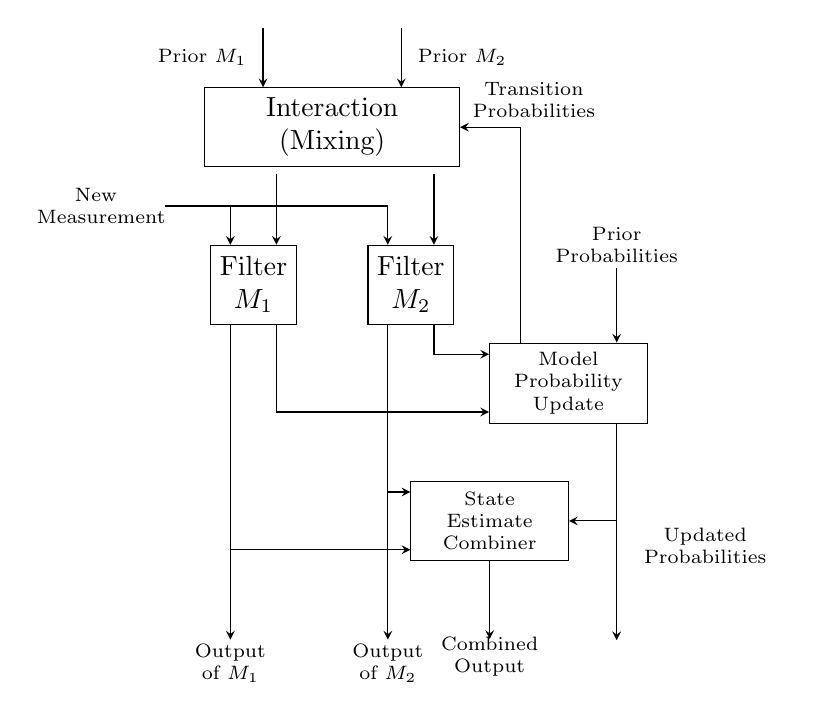
\begin{tikzpicture}[xscale=1,yscale=1,
	square/.style={rectangle, minimum height=10mm, draw=black, align=center},
	round/.style={circle, inner sep=0pt, fill=red!50, opacity=0.75, align=center},
	point/.style={circle, inner sep=0pt, minimum size=2mm, align=center},
	oval/.style={ellipse, fill=gray!50, opacity=0.75},
	label/.style={text width=5mm, align=center, font=\scriptsize},
	node distance= 3cm and 1cm, >=stealth]
	
	%Nodes
	\node[square, text width=30mm]	(interact)	at (0,0) {Interaction\\(Mixing)};
	\node[square]	(m1)	at	(-1,-2)	{Filter\\$M_1$};
	\node[square]	(m2)	at	(1,-2)	{Filter\\$M_2$};
	\node[square, minimum width=20mm, font=\scriptsize]	(prob)	at	(3,-3.25)	{Model\\Probability\\Update};
	\node[square, minimum width=20mm, font=\scriptsize]	(combine)	at	(2,-5)	{State\\Estimate\\Combiner};
	
	
	%Labels
	\node[label, text width=15mm]	(label1)	at (-3,-1)	{New\\Measurement};
	
	%Lines
	\draw[black, <-] (m1.60) -- ++(0,0.9);
	\draw[black, <-] (m2.60) -- ++(0,0.9);
	\draw[black, <-] (interact.30) -- node[label, right, xshift=-10, text width=20mm] {Prior $M_2$} ++(0,0.75);
	\draw[black, <-] (interact.150) -- node[label, left, xshift=10, text width=20mm] {Prior $M_1$} ++(0,0.75);
	\draw[black, ->] (label1.east) -| (m1.120);
	\draw[black, ->] (label1.east) -| (m2.120);
	\draw[black, ->] (m1.300) |- (prob.200);
	\draw[black, ->] (m2.300) |- (prob.160);
	\draw[black, ->] (m1.240) |- (combine.200);
	\draw[black, ->] (m2.240) |- (combine.160);
	\draw[black, ->] (prob.320) |- (combine);
	\draw[black, ->] (prob.140) |- node[label, above, xshift=5, text width=20mm] {Transition\\ Probabilities} (interact.east);
	\draw[black, <-] (prob.40) -- node[label, above, yshift=12, text width=20mm] {Prior\\Probabilities} ++(0,0.95);
	\draw[black, ->] (prob.320) -- node[label, right, yshift=-5, text width=20mm] {Updated Probabilities} ++(0,-2.75);
	
	\draw[black, ->] (m1.240) -- node[label, below, yshift=-55, text width=10mm] {Output of $M_1$} ++(0,-4);
	\draw[black, ->] (m2.240) -- node[label, below, yshift=-55, text width=10mm] {Output of $M_2$} ++(0,-4);
	\draw[black, ->] (combine) -- node[label, below, yshift=-10, text width=20mm] {Combined Output} ++(0,-1.5);
\end{tikzpicture}